\chapter{Work Plan}%
\label{chapter:workPlan}

\begin{introduction}
In this chapter, i will explain the work plan for the development of the applications and the writing of the dissertation.
\end{introduction} 


\section{Work Plan}

In the next few month i will develop the first version of the applications according to the use cases i defined in the chapter III. 
I will write the dissertation document along the way, since there may be the ocurrence of a new study or paper about this context.
The overall work plan is listed below:  

\begin{itemize}
  \item Integration with the Sytem;
  \begin{itemize}
      \item Start Date: 24/01/2025 
      \item End Date: 27/01/2025 
  \end{itemize}
    \item Receptionist use Cases;
    \begin{itemize}
        \item Start Date: 28/01/2025 
        \item End Date: 06/02/2025 
    \end{itemize}
    \item Mecanic Use Cases;
    \begin{itemize}
      \item Start Date: 07/02/2025 
      \item End Date: 13/03/2025 
  \end{itemize}
    \item Admin Use Cases;
    \begin{itemize}
      \item Start Date: 14/03/2025 
      \item End Date: 06/04/2025 
  \end{itemize}
    \item Warehouse Use Cases;
    \begin{itemize}
      \item Start Date: 07/04/2025 
      \item End Date: 11/04/2025 
  \end{itemize}
    \item Client App;
    \begin{itemize}
      \item Start Date: 12/04/2025 
      \item End Date: 03/05/2025 
  \end{itemize}
  \item User Testing;
  \begin{itemize}
    \item Start Date: 04/05/2025 
    \item End Date: 11/05/2025 
\end{itemize}
  \item Apply suggestion;
  \begin{itemize}
    \item Start Date: 12/05/2025 
    \item End Date: 25/05/2025 
\end{itemize}
  \end{itemize}

  Following de development of the applications, i will reserve a week to conduct a user testing with preferelly users related to the subject and another week to apply the notes and suggestion the experiment provided to the application.
  The remaining time will use to finish writing the dissertation, primarly the results and conclusion.
  The literature will accompany all of this proccess, since it may appear another paper or study that my be relevant to my work.
  This information is illustrated in figure \ref{fig:figure1}.

    \begin{figure}[h]
      \caption{Planned Work described as a Gantt Chart. The master thesis is estimated to be at 25\%, the literature progress to be 80\%, the application Use cases at 85\% and the admin Use Cases at 10\%.}
      \centering
      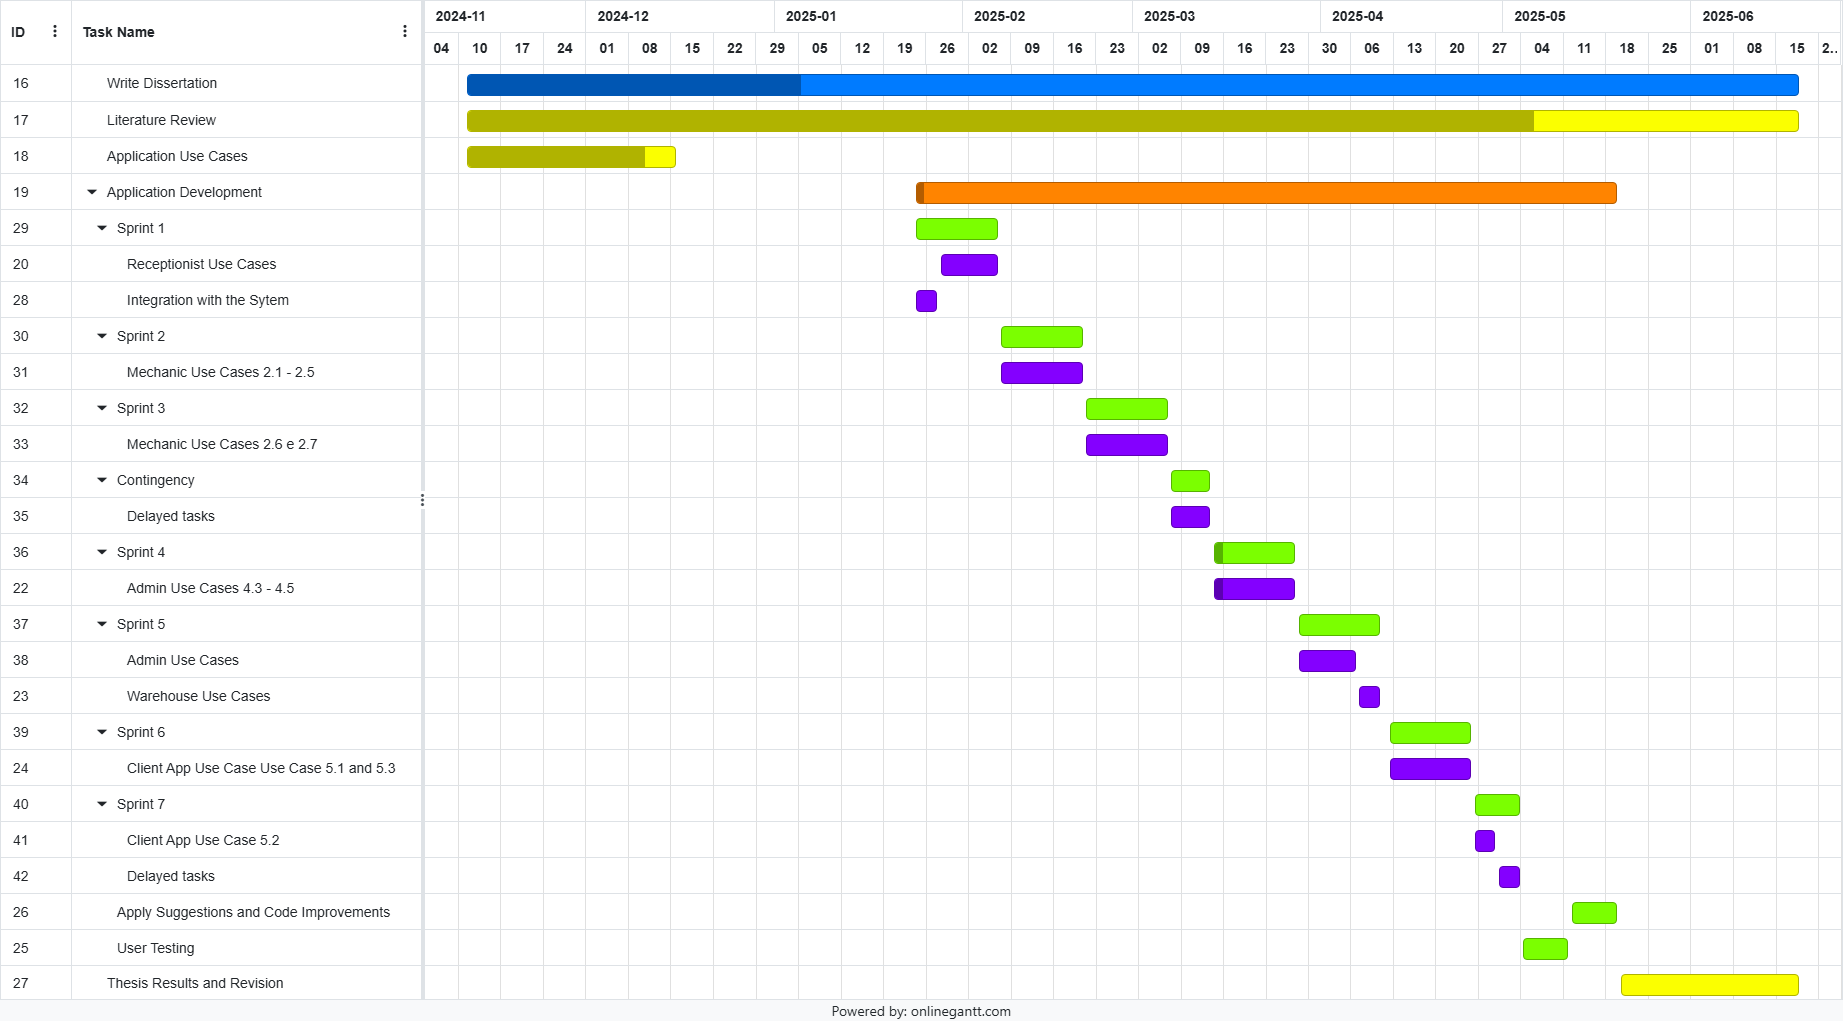
\includegraphics[width=\textwidth]{figs/Gantt}
      \label{fig:figure1}
    \end{figure}
